% \documentclass[10pt, twocolumn, a4paper]{article}
\documentclass[12pt,a4paper]{article}

\usepackage[backend=biber, style=ieee]{biblatex}                        % To include the bibliography
\usepackage[left=2cm, right=2cm, top=2.5cm, bottom=2.5cm]{geometry}     % To set the margins
\usepackage[noend]{algpseudocode}
\usepackage[table]{xcolor}                                              % For coloring cells

\usepackage{algorithm}                                                  % To include algorithms
\usepackage{amsfonts}                                                   % To include math fonts:ToggleTerm direction=float
\usepackage{amsmath}                                                    % To include Mathematic symbols
\usepackage{authblk}                                                    % To format author affiliations
\usepackage{caption}                                                    % For caption spacing
\usepackage{float}                                                      % To place figures where you want them
\usepackage{graphicx}                                                   % To include images
\usepackage{hyperref}                                                   % To include hyperlinks
\usepackage{lipsum}                                                     % TODO: remove this
\usepackage{listings}                                                   % To include code
\usepackage{tabularx}                                                   % For equal-width columns
\usepackage{tcolorbox}                                                  % To make colored boxes
\usepackage{tikz}                                                       % To draw graphs
\usepackage{titlesec}                                                   % To format section titles
\usepackage{xcolor}                                                     % To define colors

\usetikzlibrary{graphs,graphs.standard}
\usetikzlibrary{positioning}

\addbibresource{./references.bib}

% Esto es para poder hacer cajitas de código con el fondo gris
\lstset{
    language=C++,
    basicstyle=\ttfamily\small,
    keywordstyle=\color{blue}\bfseries,
    stringstyle=\color{green!60!black},
    commentstyle=\color{gray},
    backgroundcolor=\color{gray!05},
    frame=single,
    numbers=left,
    numberstyle=\small,
    stepnumber=1,
    numbersep=10pt,
    tabsize=2,
    showstringspaces=false,
    captionpos=b,
}

% Para poder hacer flechas
\usetikzlibrary{shapes, arrows}

% Sección de definiciones
\titleformat{\section}{\Large\bfseries}{\thesection}{1em}{}
\titleformat{\subsection}{\large\bfseries}{\thesubsection}{1em}{}

% Caja de colores
\definecolor{mint}{RGB}{202,251,202}
\definecolor{yellow}{RGB}{255,255,202}
\definecolor{red}{RGB}{255,202,202}

% Variables globales
\newcommand{\currentsemester}{Segundo Semestre}
\newcommand{\currentyear}{2025}


\begin{document}

\begin{center}
    \LARGE\textbf{Programación Paralela} \\
    \Large{Teórica 02 - Introducción a CUDA} \\
    \normalsize{Segundo Semestre, 2025} \\
    \vspace{1em}
    \hrule
\end{center}

\section*{Introducción}

Para los ejercicios vamos a hacer CUDA C que nos permite escribir programas paralelos escalables en sistemas paralelos
donde conviven tanto CPUs como GPUs. \textbf{En este tipo de sistemas donde hay porciones de código que pueden
ejecutarse en paralelo, pero que están gobernadas por un código secuencial que corre en la CPU, los llamaremos
\textit{heterogéneos}.} CUDA extiende el lenguaje de programación C con una sintaxis mínima que permite realizar tanto
sistemas conteniendo CPUs o GPUs.

Cuando en el software moderno las aplicaciones se ejecutan \textit{lento}, el problema usualmente suele ser que hay
demasiados datos para ser procesados. Por ejemplo casos como el procesamiento de imágenes o videos, simulación de
dinámica de fluidos, manejo de sistemas complejos como (líneas aéreas), o incluso cosas mucho más sencillas como
convertir una imagen de pixels a escala de grises, se pueden fraccionar en tareas más pequeñas que pueden ser ejecutadas
de manera independiente.

\begin{tcolorbox}[colback=yellow,colframe=yellow!75!black,arc=0pt,outer arc=0pt]
  \textbf{Paralelismo de tareas vs. paralelismo de datos} \\

  El paralelismo de tareas se refiere a la ejecución de múltiples tareas (no necesariamente las mismas) al mismo tiempo.
  Por otro lado, el paralelismo de datos se refiere a la ejecución de la misma tarea en múltiples datos al mismo tiempo.
\end{tcolorbox}


\section*{Convertir una Imagen a Escala de Grises}

El procesamiento de imágenes es un clásico ejemplo de computación paralela y lo utilizaremos mucho durante la materia
para ejemplificar conceptos. En este caso vamos a ver cómo convertir una imagen a escala de grises.

Pero antes de comenzar tenemos que saber cómo se representa una imagen en la computadora. Esencialmente una imagen se
puede representar como una matriz de tuplas $(R, G, B)$ donde $R$, $G$ y $B$ son los valores de los colores rojo, verde
y azul respectivamente. Cada uno de estos valores puede ir desde 0 a 255 y representan la intensidad de cada color en un
pixel. Esa combinación se encuentra dentro del triángulo AdobeRGB (ver Figura \ref{fig:adobe_rgb}).

\begin{figure}[H]
  \centering
  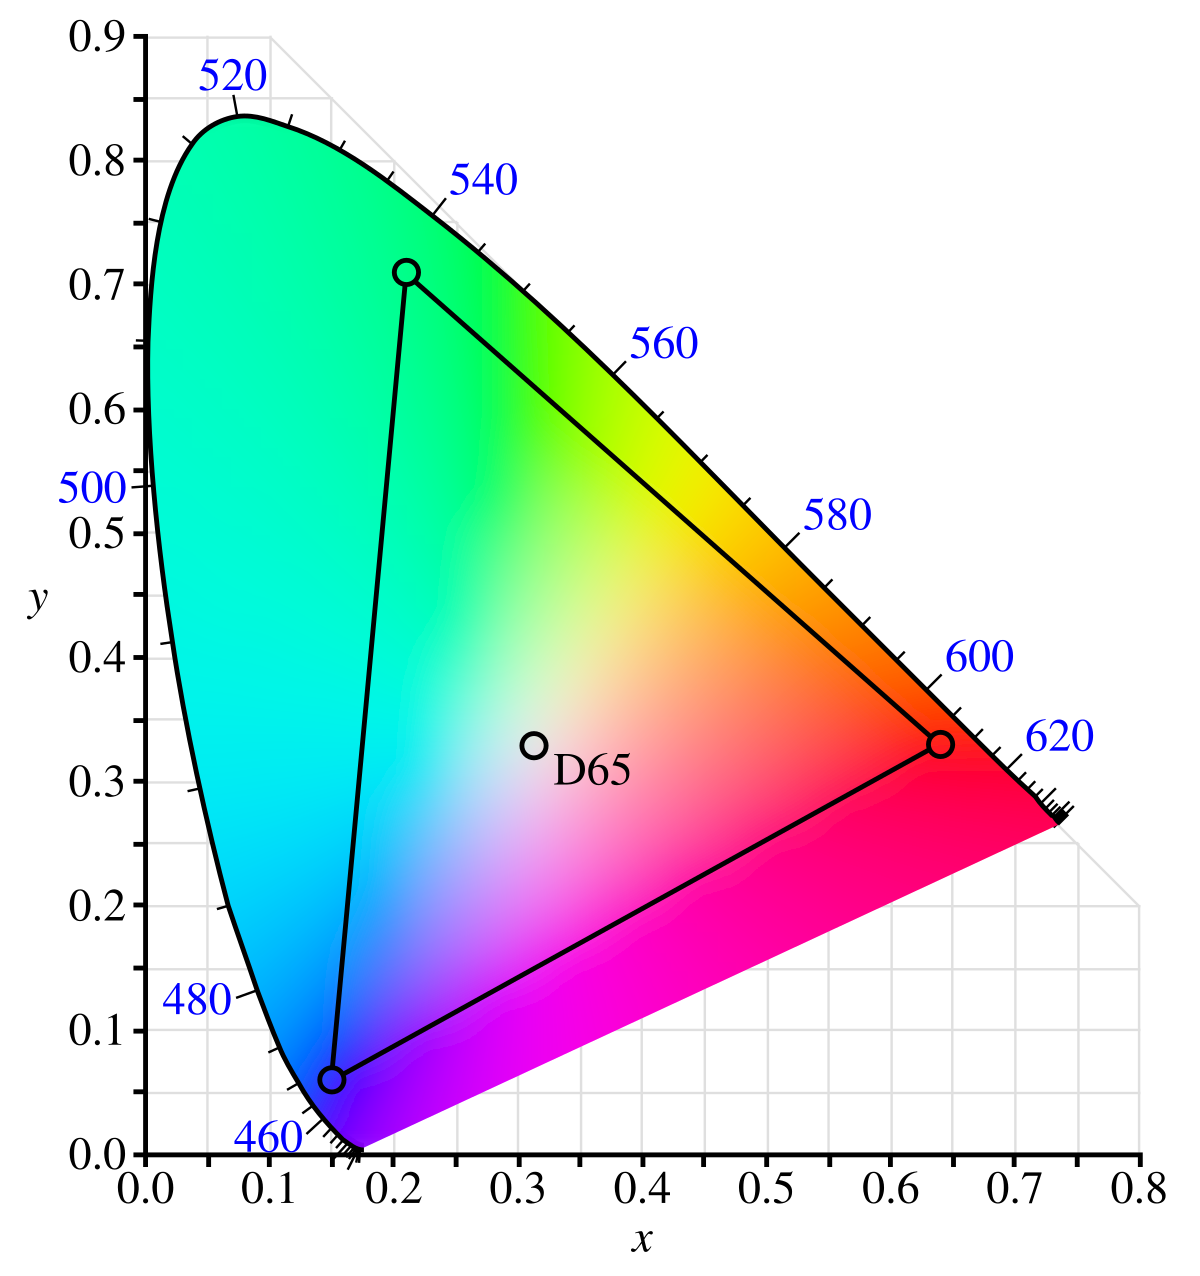
\includegraphics[width=200px]{./images/adobe_rgb.png}
  \caption{Triángulo AdobeRGB}
  \label{fig:adobe_rgb}
\end{figure}

Estos valores $R$, $G$ y $B$ representan los \textit{canales} y para convertir estos canales a escala de grises se debe
utilizar una fórmula, ya que hay que decidir cuál va a ser la intensidad del pixel en escala de grises. Esto se hace
combinando los valores de los canales de color de alguna manera. Lógicamente hay muchas formas de convertir estos
canales a escala de grises, por ejemplo podríamos tomar sólo el valor del canal $G$, pero la imagen sólo se vería
representada en una escala de grises para el canal verde, lo cual no sería muy verídico. Sin embargo si lo pensamos no
es trivial cuál es la fórmula para traducir una imagen de color a escala de grises. \\

\begin{tcolorbox}[colback=mint,colframe=yellow!75!black,arc=0pt,outer arc=0pt]
  \textbf{Fórmulas para convertir a escala de grises} \\

  \begin{itemize}
    \item \textbf{Promedio}: $I = \frac{R + G + B}{3}$
    \item \textbf{Luminosidad}: $I = 0.21R + 0.72G + 0.07B$
    \item \textbf{Desaturación}: $I = \frac{max(R, G, B) + min(R, G, B)}{2}$
  \end{itemize}
\end{tcolorbox}

En este caso usaremos la fórmula de \textit{luminosidad} para convertir la imagen a escala de grises que es un promedio
pesado de los canales de color que representa la percepción humana de la luminosidad, pero como dijimos no es la única
forma y cambiar esta fórmula puede dar diferentes resultados que podrían considerarse como "filtros de imagen" (¡podés
probarlo luego!).


\section*{Estructura de un programa en CUDA C}

La estructura de un programa en CUDA C es similar a un programa en C, lo que refleja su naturaleza heterogénea donde
existe un \textit{host} (CPU) y uno o más \textit{devices} (GPU) en la computadora. El código fuente CUDA tiene una
mezcla de ambos códigos, uno que se ejecuta en el host y otro en el device. Por defecto, todo el código se ejecuta en el
host. Las funciones declaradas para ser corridas en los \textit{devices} son aquellas que exhibirán una gran cantidad de
paralelismo de datos.

El código con estas extensiones de CUDA tiene que ser compilado con el compilador de NVIDIA, \texttt{nvcc}, que es un
wrapper para el compilador de C, \texttt{gcc}. El compilador de NVIDIA se encarga de separar el código que se ejecuta en
el host del que se ejecuta en el device y de compilarlo con el compilador de C. El código identificado con las
\textit{keywords} (palabras reservadas) de CUDA para las funciones paralelas se denominan \textit{kernels}. Estos
kernels son funciones que están asociadas a estructuras de datos y que van a ser ejecutadas en paralelo por GPUs. En las
situaciones donde no haya una GPU disponible, el código de todas formas se ejecutará en una CPU (uno podría incluso
ejecuar el kernel en CPU utilizando herramientas como MCUDA) \cite{sutter2005}.

\newpage

\vspace{1em}

\printbibliography


\end{document}
